%!TEX root = ./icml2016.tex
\section{Experiments}
\subsection{Synthetic data}
\begin{figure}[t]
	\centering
	
	\subfigure[E=5, K=5, D=5\label{fig:syn1}]{
	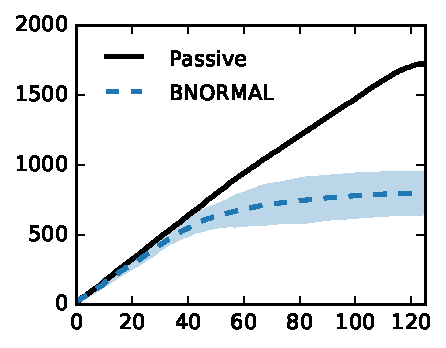
\includegraphics[width=0.42\linewidth]{images/toy_5_5_5.pdf}
	}
	\subfigure[E=10, K=10, D=5\label{fig:syn2}]{
	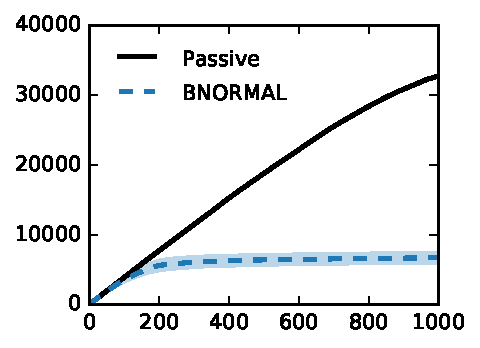
\includegraphics[width=0.45\linewidth]{images/toy_10_10_5.pdf}				
	}
%	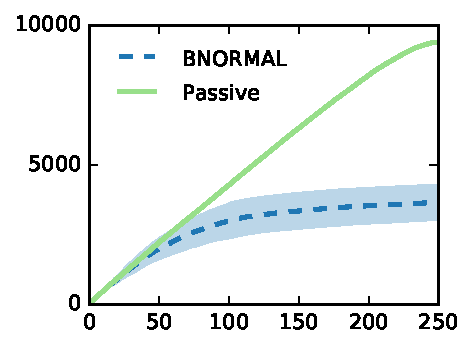
\includegraphics[width=0.32\linewidth]{images/toy_5_10_5.pdf}			
%	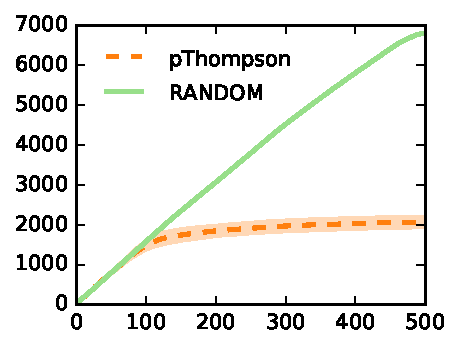
\includegraphics[width=0.32\linewidth]{images/toy_10_5_5.pdf}				
	\caption{\label{fig:synthetic} Cumulative regret of particle Thompson sampling on different sizes of the synthetic dataset. The synthetic dataset is generated by the model assumption (Eq. \ref{eqn:entity_gen} - \ref{eqn:triple_gen}). We compared the particle Thompson sampling with random sampling method. The averaged cumulative regrets are plotted with one standard error. As the model obtained more and more labeled samples from Thompson sampling, the cumulative regrets are converged. This result  indicates the particle sampling correctly inferred latent features of entities and relations on the synthetic datasets. // The results are averaged over 10 runs. $\sigma_e = 10$, $\sigma_r=10$, $\sigma_x=0.1$, $H=5$.}
\end{figure}

\subsection{Synthetic data}
\begin{figure}[t]
	\centering
	
	\subfigure[KINSHIP]{
	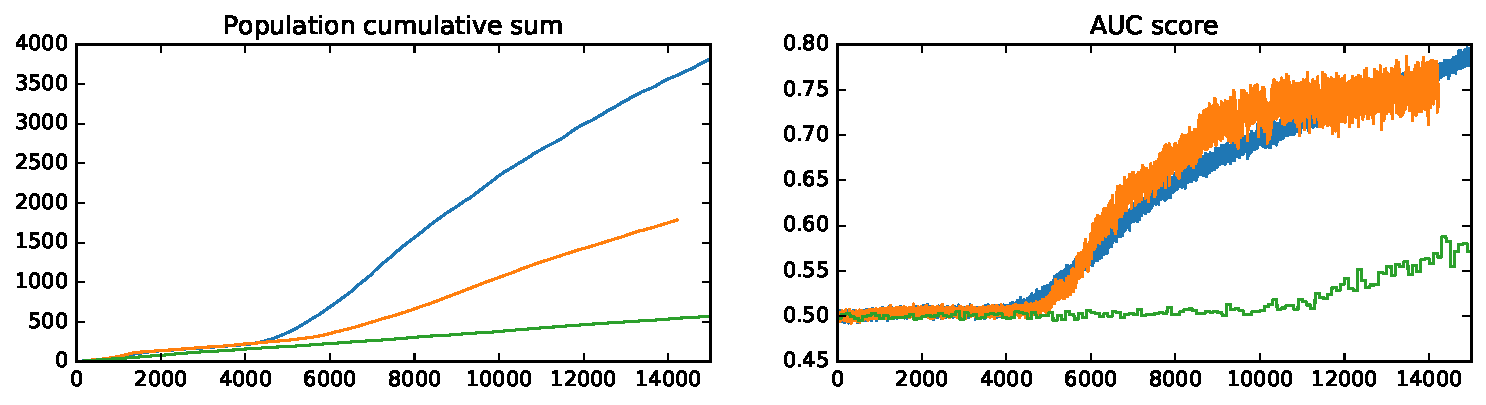
\includegraphics[width=\linewidth]{images/thompson_kinship.pdf}
	}
	\subfigure[UMLS]{
	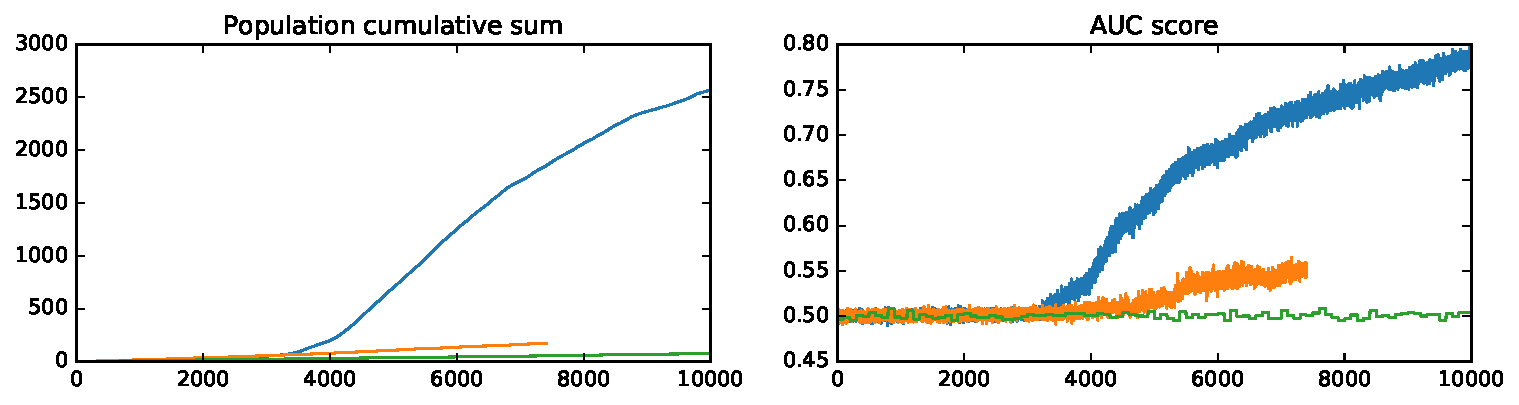
\includegraphics[width=\linewidth]{images/thompson_umls.pdf}				
	}
	\subfigure[NATION]{
	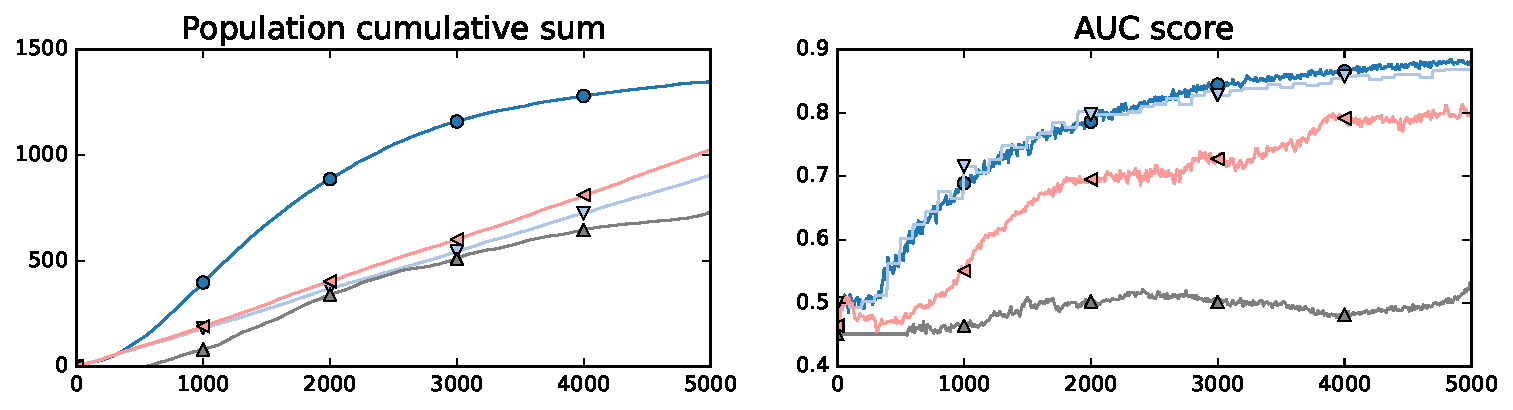
\includegraphics[width=\linewidth]{images/thompson_nation.pdf}				
	}	
	\caption{Placeholder for the future results. Will include the cumulative gain and ROC-AUC score of the developed models with the active and passive learning methods. We will see how the compositional model performs to compare with other models without any initial observation (May include the IBM model without any initial observation).}
\end{figure}

\section{Unstructured thoughts}

\begin{description}
  \item[Not useful theorem] In \cite{kawale2015efficient}, the theorem does not really give
  a setting that is used in the paper.
  \item[Logistic regression] For outputs which are binary, instead of a Gaussian assumption on
  $x$, we can use logistic regression. See
   \url{http://people.csail.mit.edu/romer/papers/TISTRespPredAds.pdf}
  \item[Choosing triples] For entity $e_i$ related via relation $R_k$ to entity $e_j$, we want
  an active learning algorithm that will choose triples $e_i R_k e_j$ that corresponds to
  $x_{ikj}$. This will not have a bandit regret bound, since we only choose each triple once.
  \item[Contextual Bandits] There are two groups of three possible assumptions for contextual
  bandits:
  \begin{enumerate}
    \item Two elements of the tuple as context, choose only one element
    \begin{itemize}
      \item $e_iR_k$ context, $e_j$ arms
      \item $e_i, e_j$ context, $R_k$ arms
      \item $R_ke_j$ context, $e_i$ arms
    \end{itemize}
    \item One element of the tuple as context, choose two elements
    \begin{itemize}
      \item $e_i$ context, $R_k e_j$ arms
      \item $R_k$ context, $e_i, e_j$ arms
      \item $e_j$ context, $e_iR_k$ arms
    \end{itemize}
  \end{enumerate}
\end{description}

\begin{table}
\centering
\caption{\label{tbl:dataset}Description of datasets.}
\begin{tabular}{l | r | r | r | r}
Dataset &  \# rel & \# entities & \# triples & sparsity \\ \hline
Kinship & 26 & 104  & 10,790 & 0.038 \\
UMLS & 49 &135  & 6,752 & 0.008 \\
Nation & 56 & 14  & 2,024 & 0.184 \\
%Wordnet & 11 & 38,696  &123,429 & 7.5e-06\\
%Wordnet(N) & 10 & 836 & 1,766 & 2.5e-04\\
\end{tabular}
\end{table}

% In the unusual situation where you want a paper to appear in the
% references without citing it in the main text, use \nocite

